\documentclass{article}
\usepackage{graphicx}
\title{Comparation of Search Engines}
\author{Xujie Yuan}
% \date{2022-09-29}
\begin{document}
    \maketitle
    \section{Introduction}
    With the development of Internet technology, the use of search engines has become an essential part of the process of learning and working. There are many well-known search engines, such as Google, Bing, Baidu. It can be said that they are commercially successful, but in the actual use of the process, I found that even for the same search content, the three search engines search results are very different, especially in the more professional scientific research, engineering field. This paper will take K-means clustering algorithm as an example to compare the search results of the three search engines.

    \section{Google search results}
    \begin{figure}[ht]
        \centering
        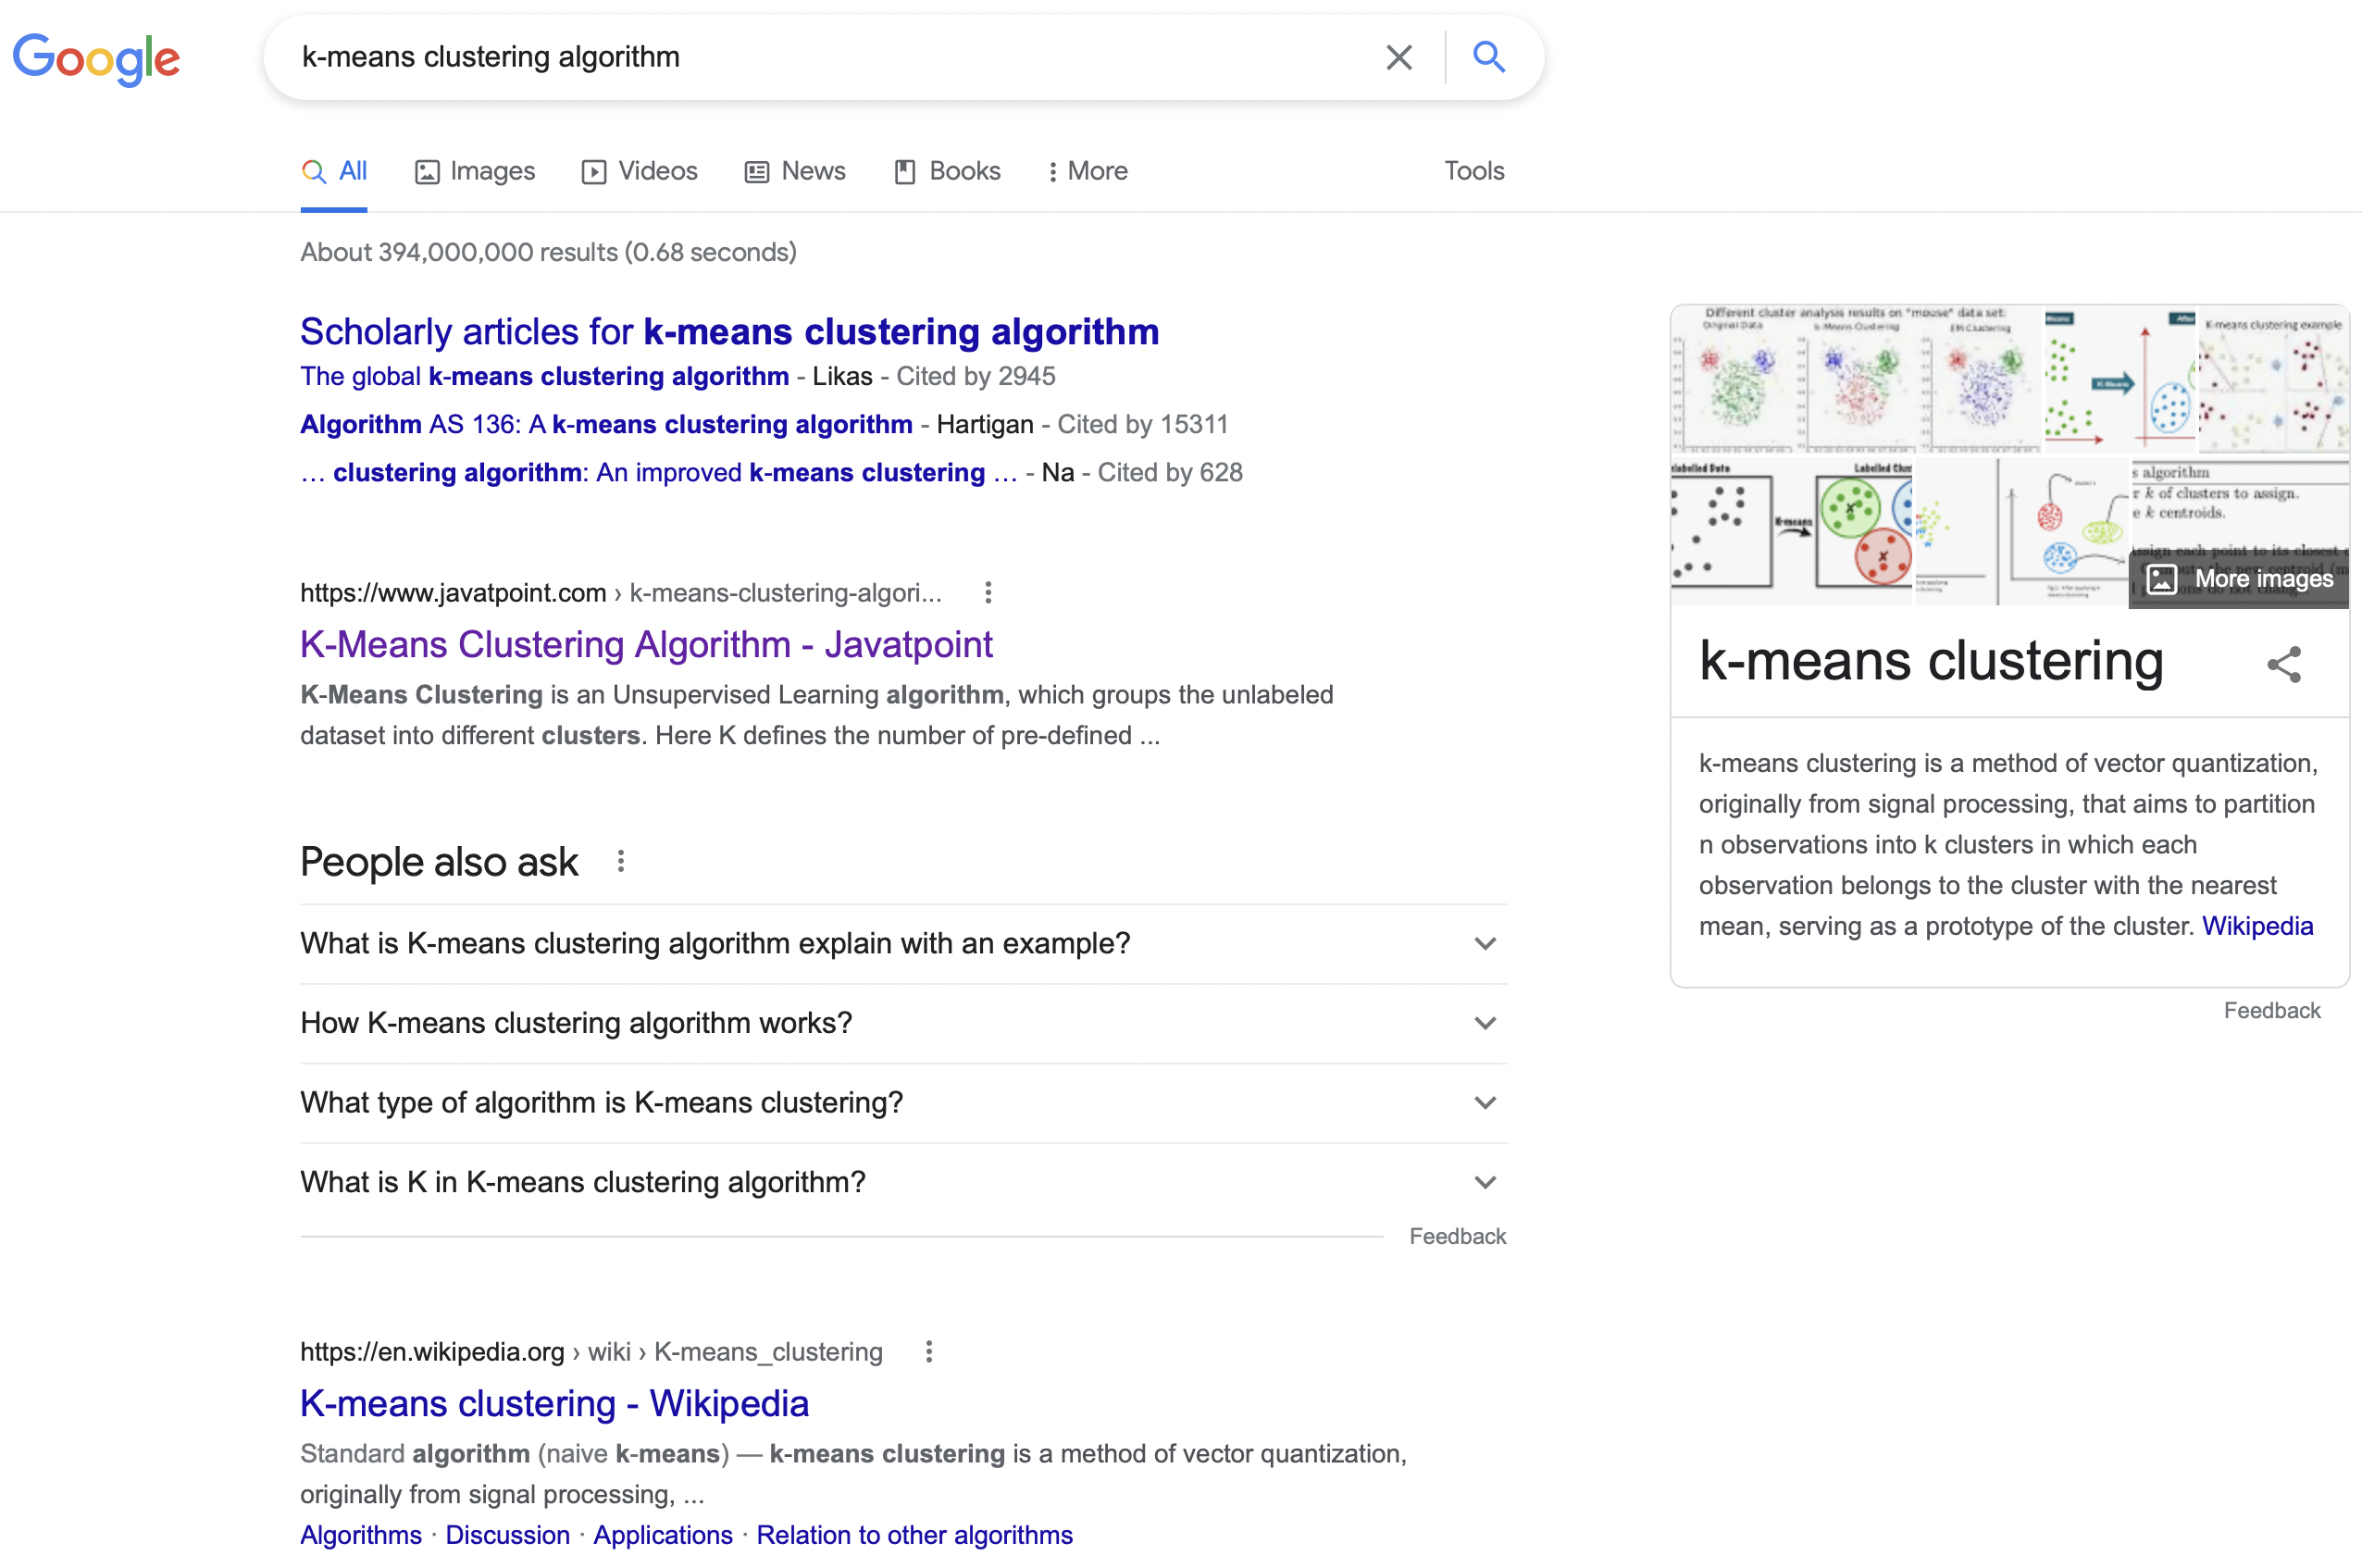
\includegraphics[width=0.8\textwidth]{Google_home.png}
        \caption{Google search results}
    \end{figure}
    As shown above, in Google's search results, there are recommended academic articles about K-means clustering algorithm at the top, and users can directly check the corresponding content, as shown in Figure 2. There is also a brief introduction to K-means clustering from Wikipedia on the right side of the interface. Users can also click on the top-ranked result, as shown in Figure 3, which contains very detailed information about the keywords. The top results are followed by other users' high-frequency searches for the keyword.
    \begin{figure}[ht]
        \centering
        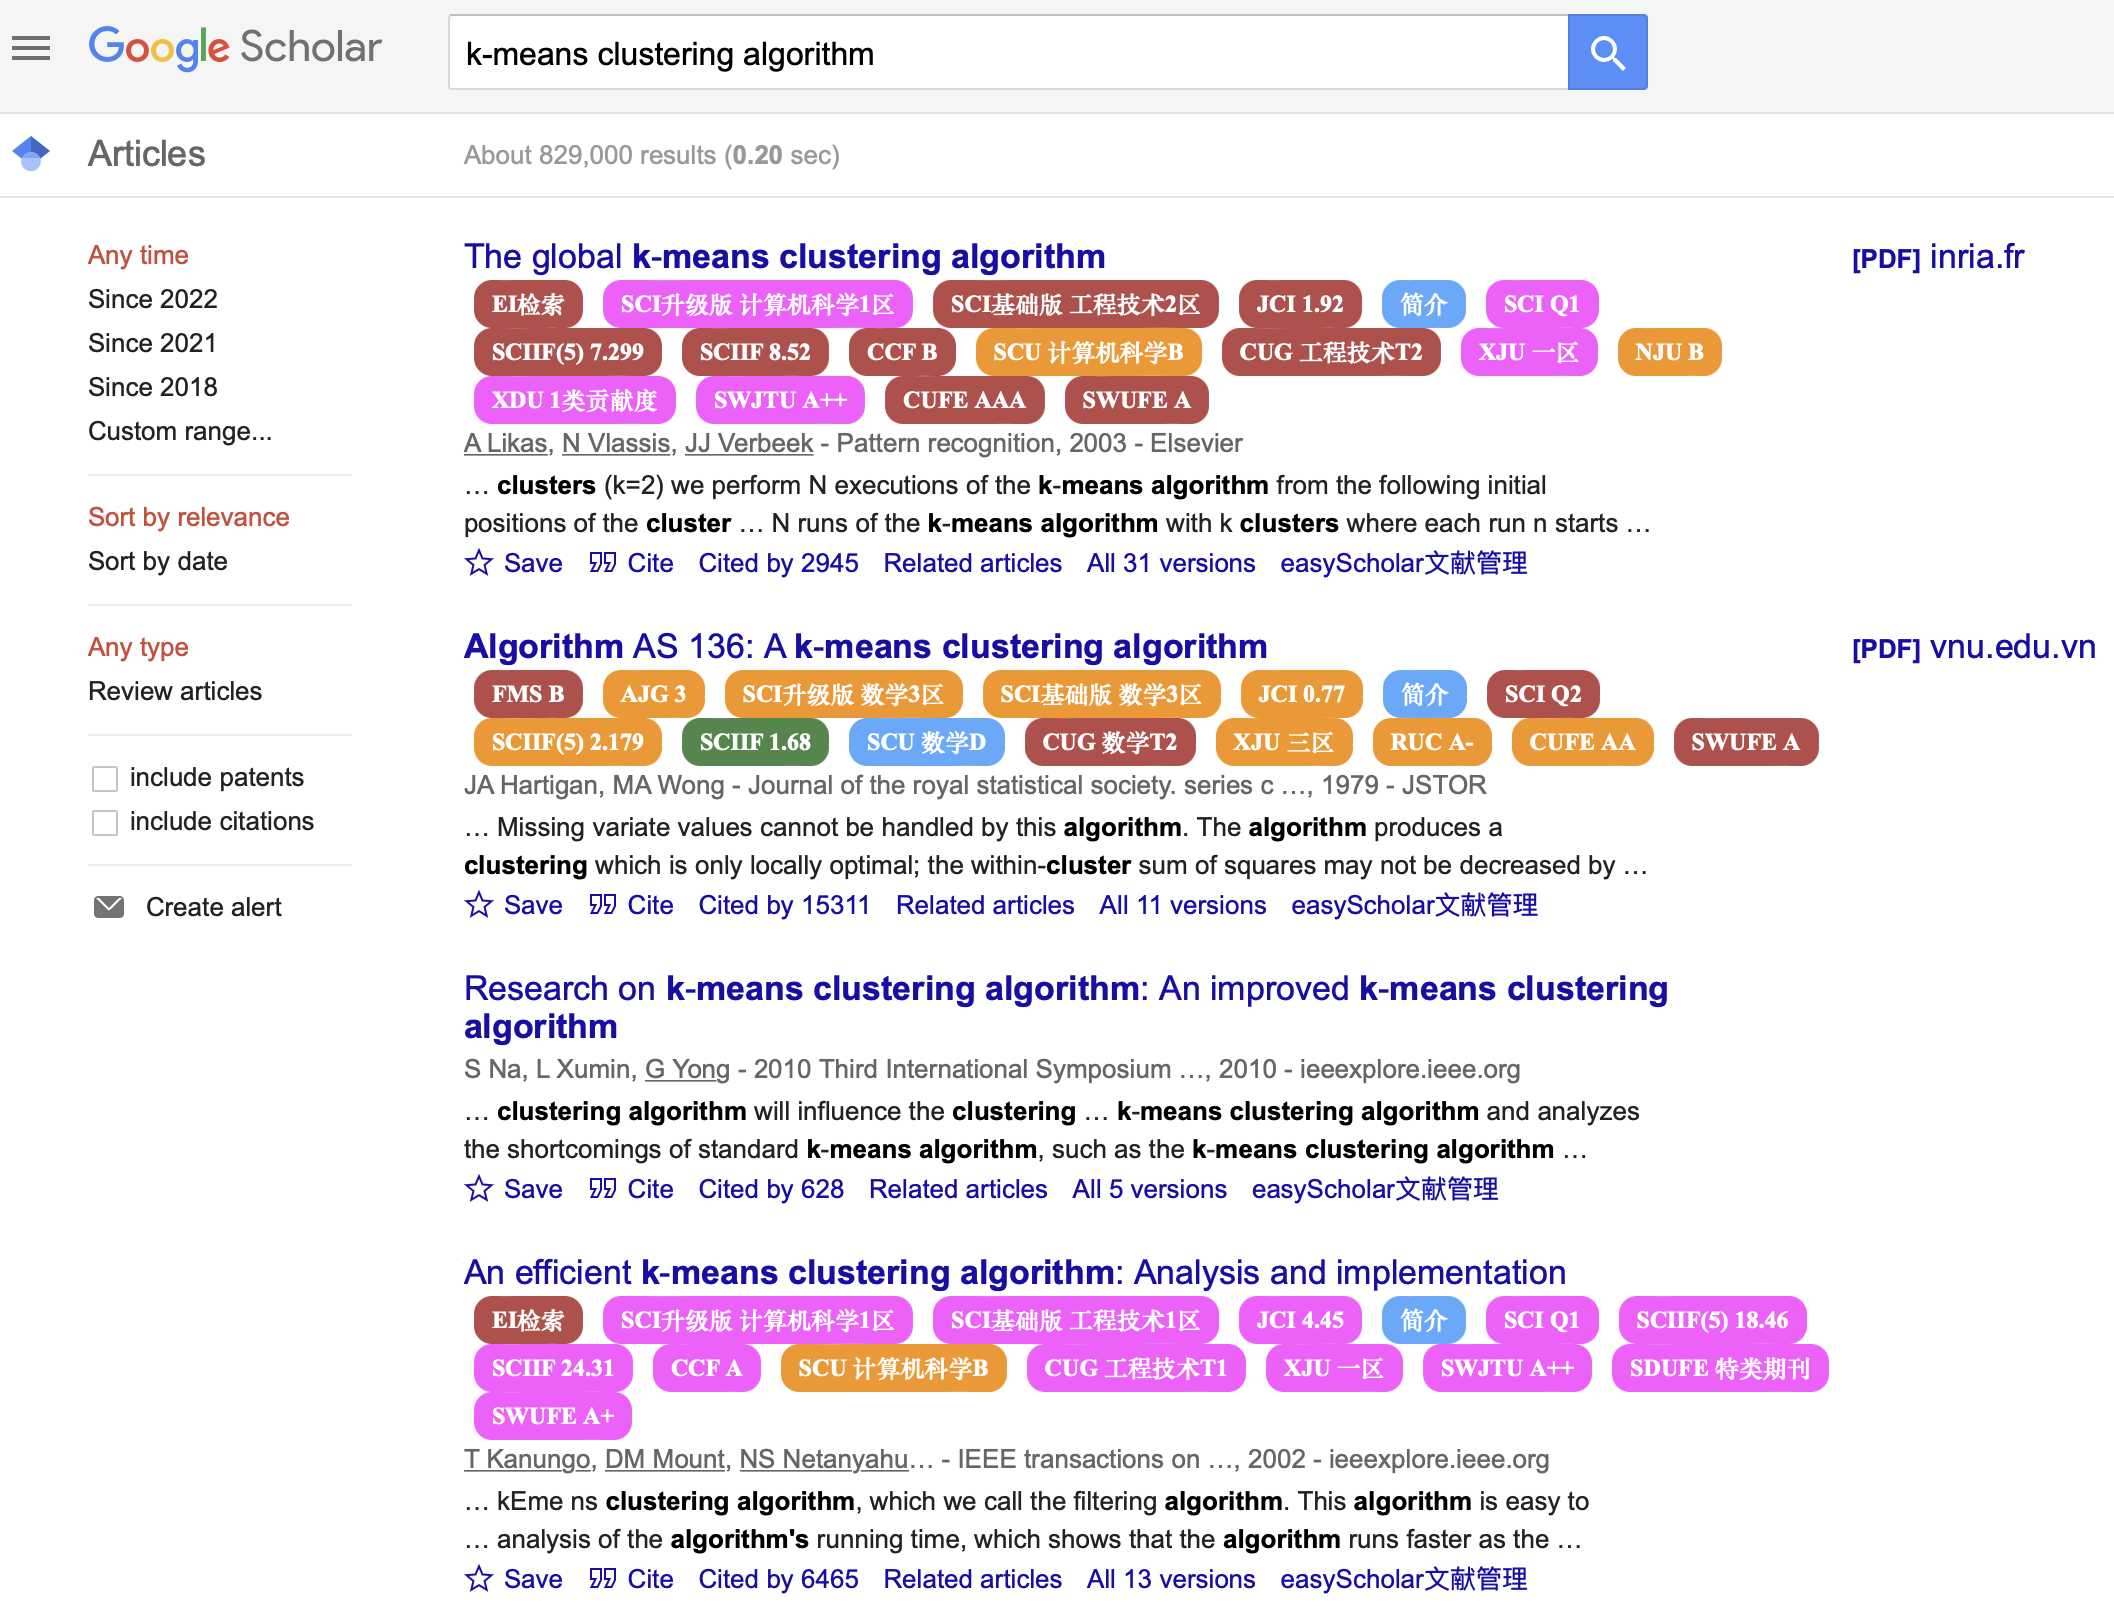
\includegraphics[width=0.8\textwidth]{googleScholar.png}
        \caption{Google Scholar results}
    \end{figure}
    \begin{figure}[ht]
        \centering
        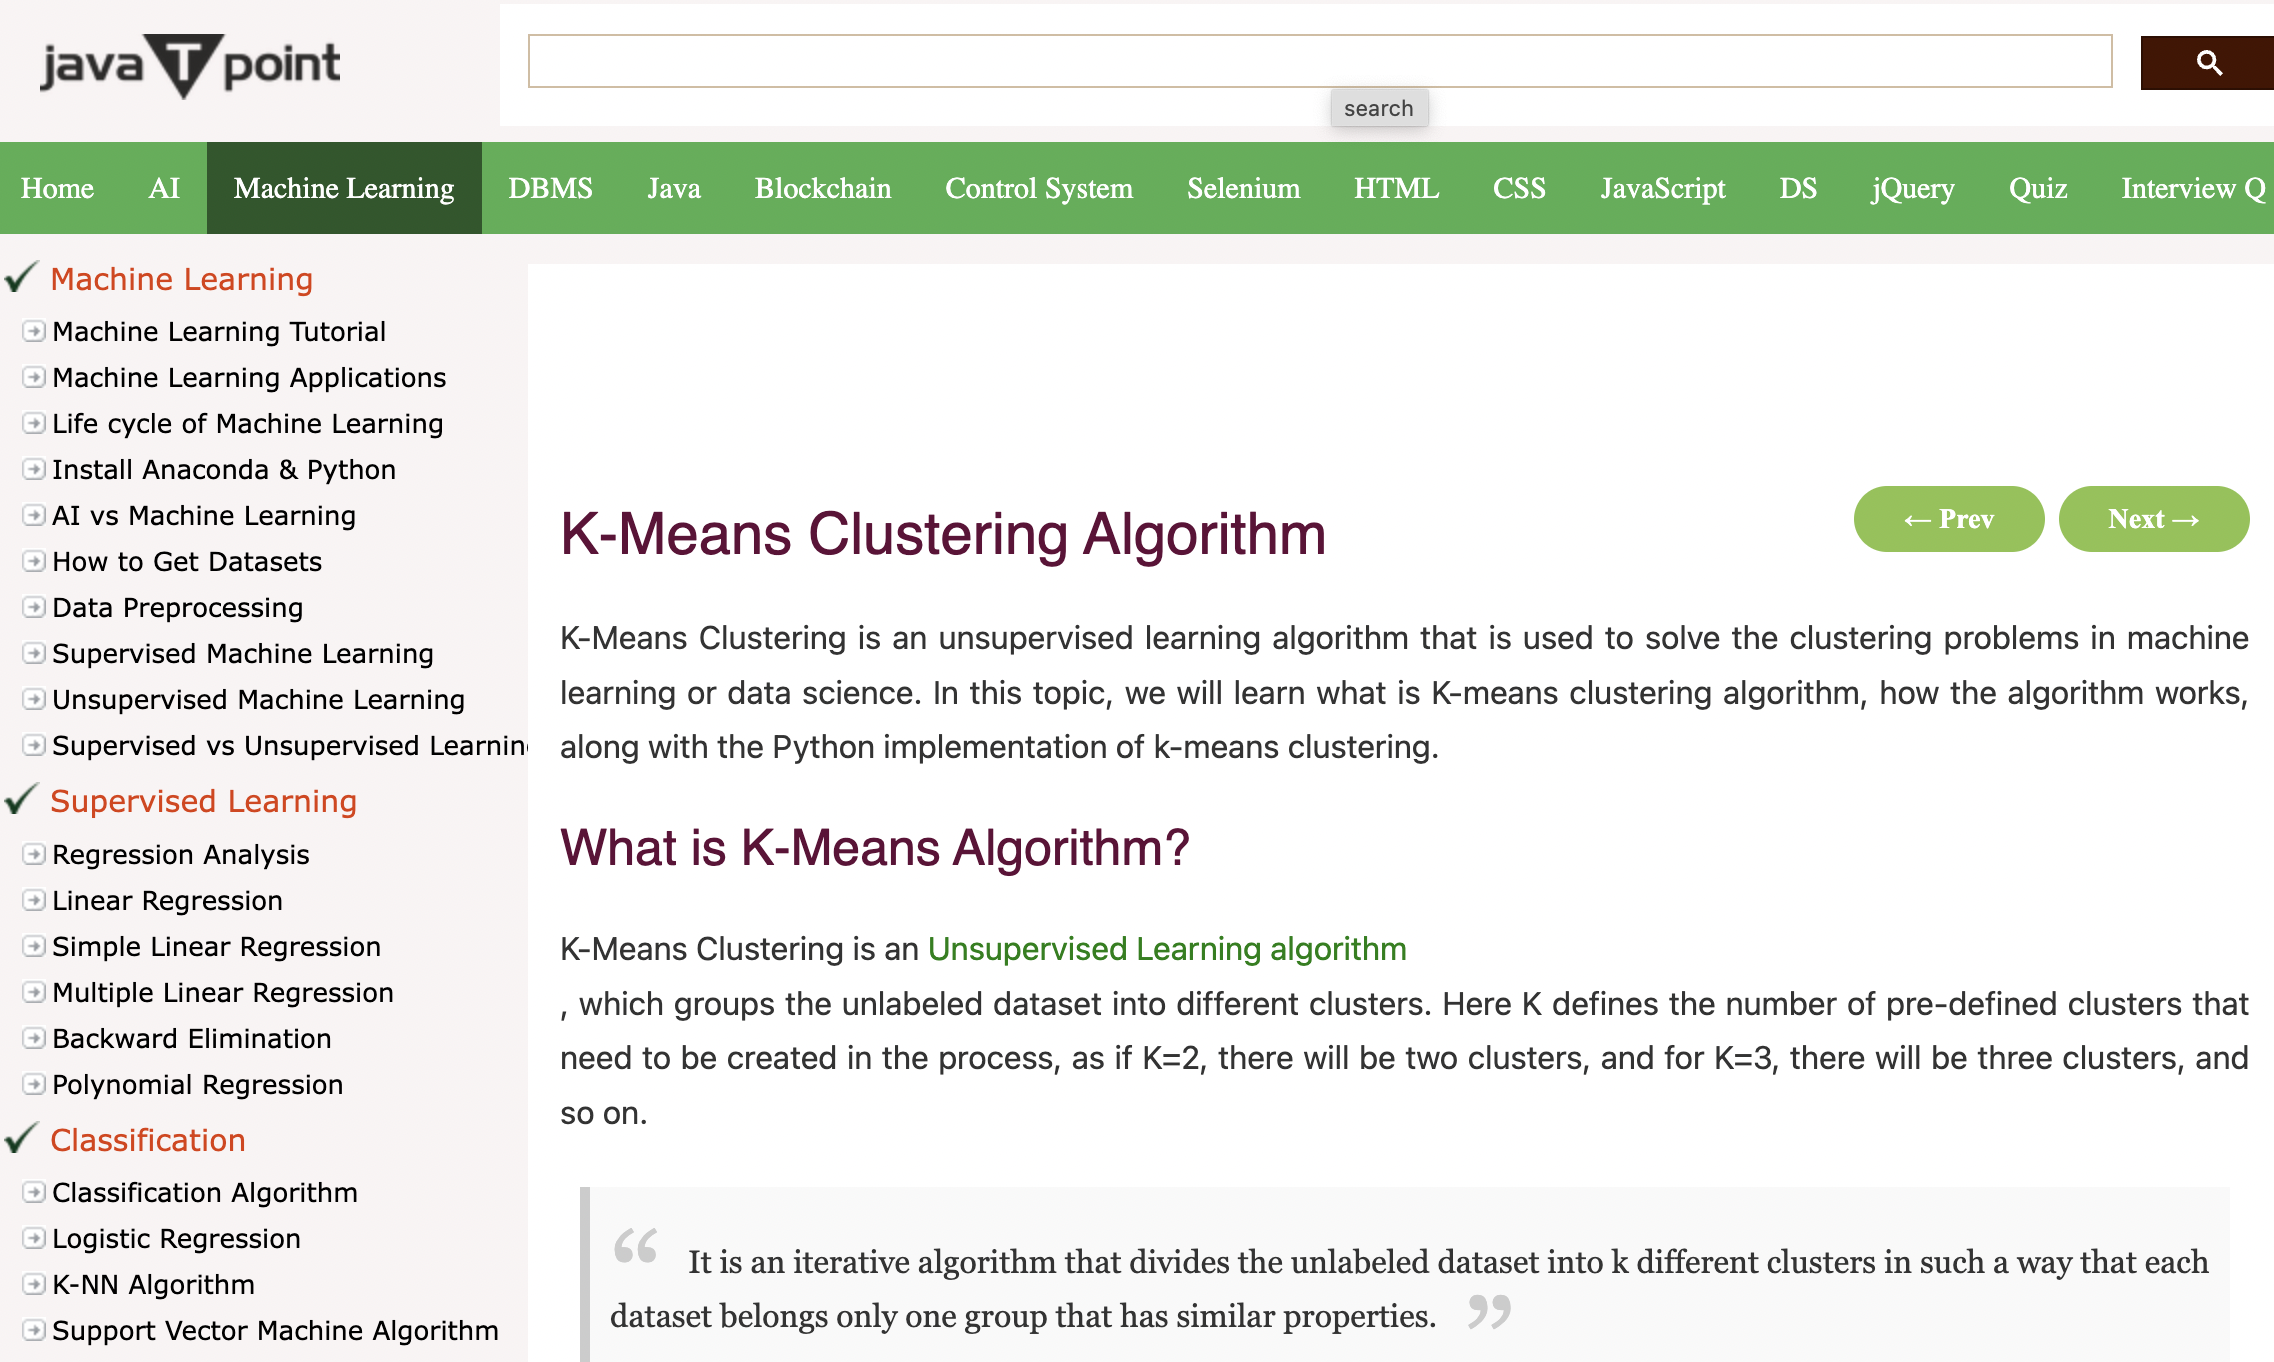
\includegraphics[width=0.8\textwidth]{google1.png}
        \caption{Google high ranked result}
    \end{figure}

    \section{Bing search results}
    \begin{figure}[ht]
        \centering
        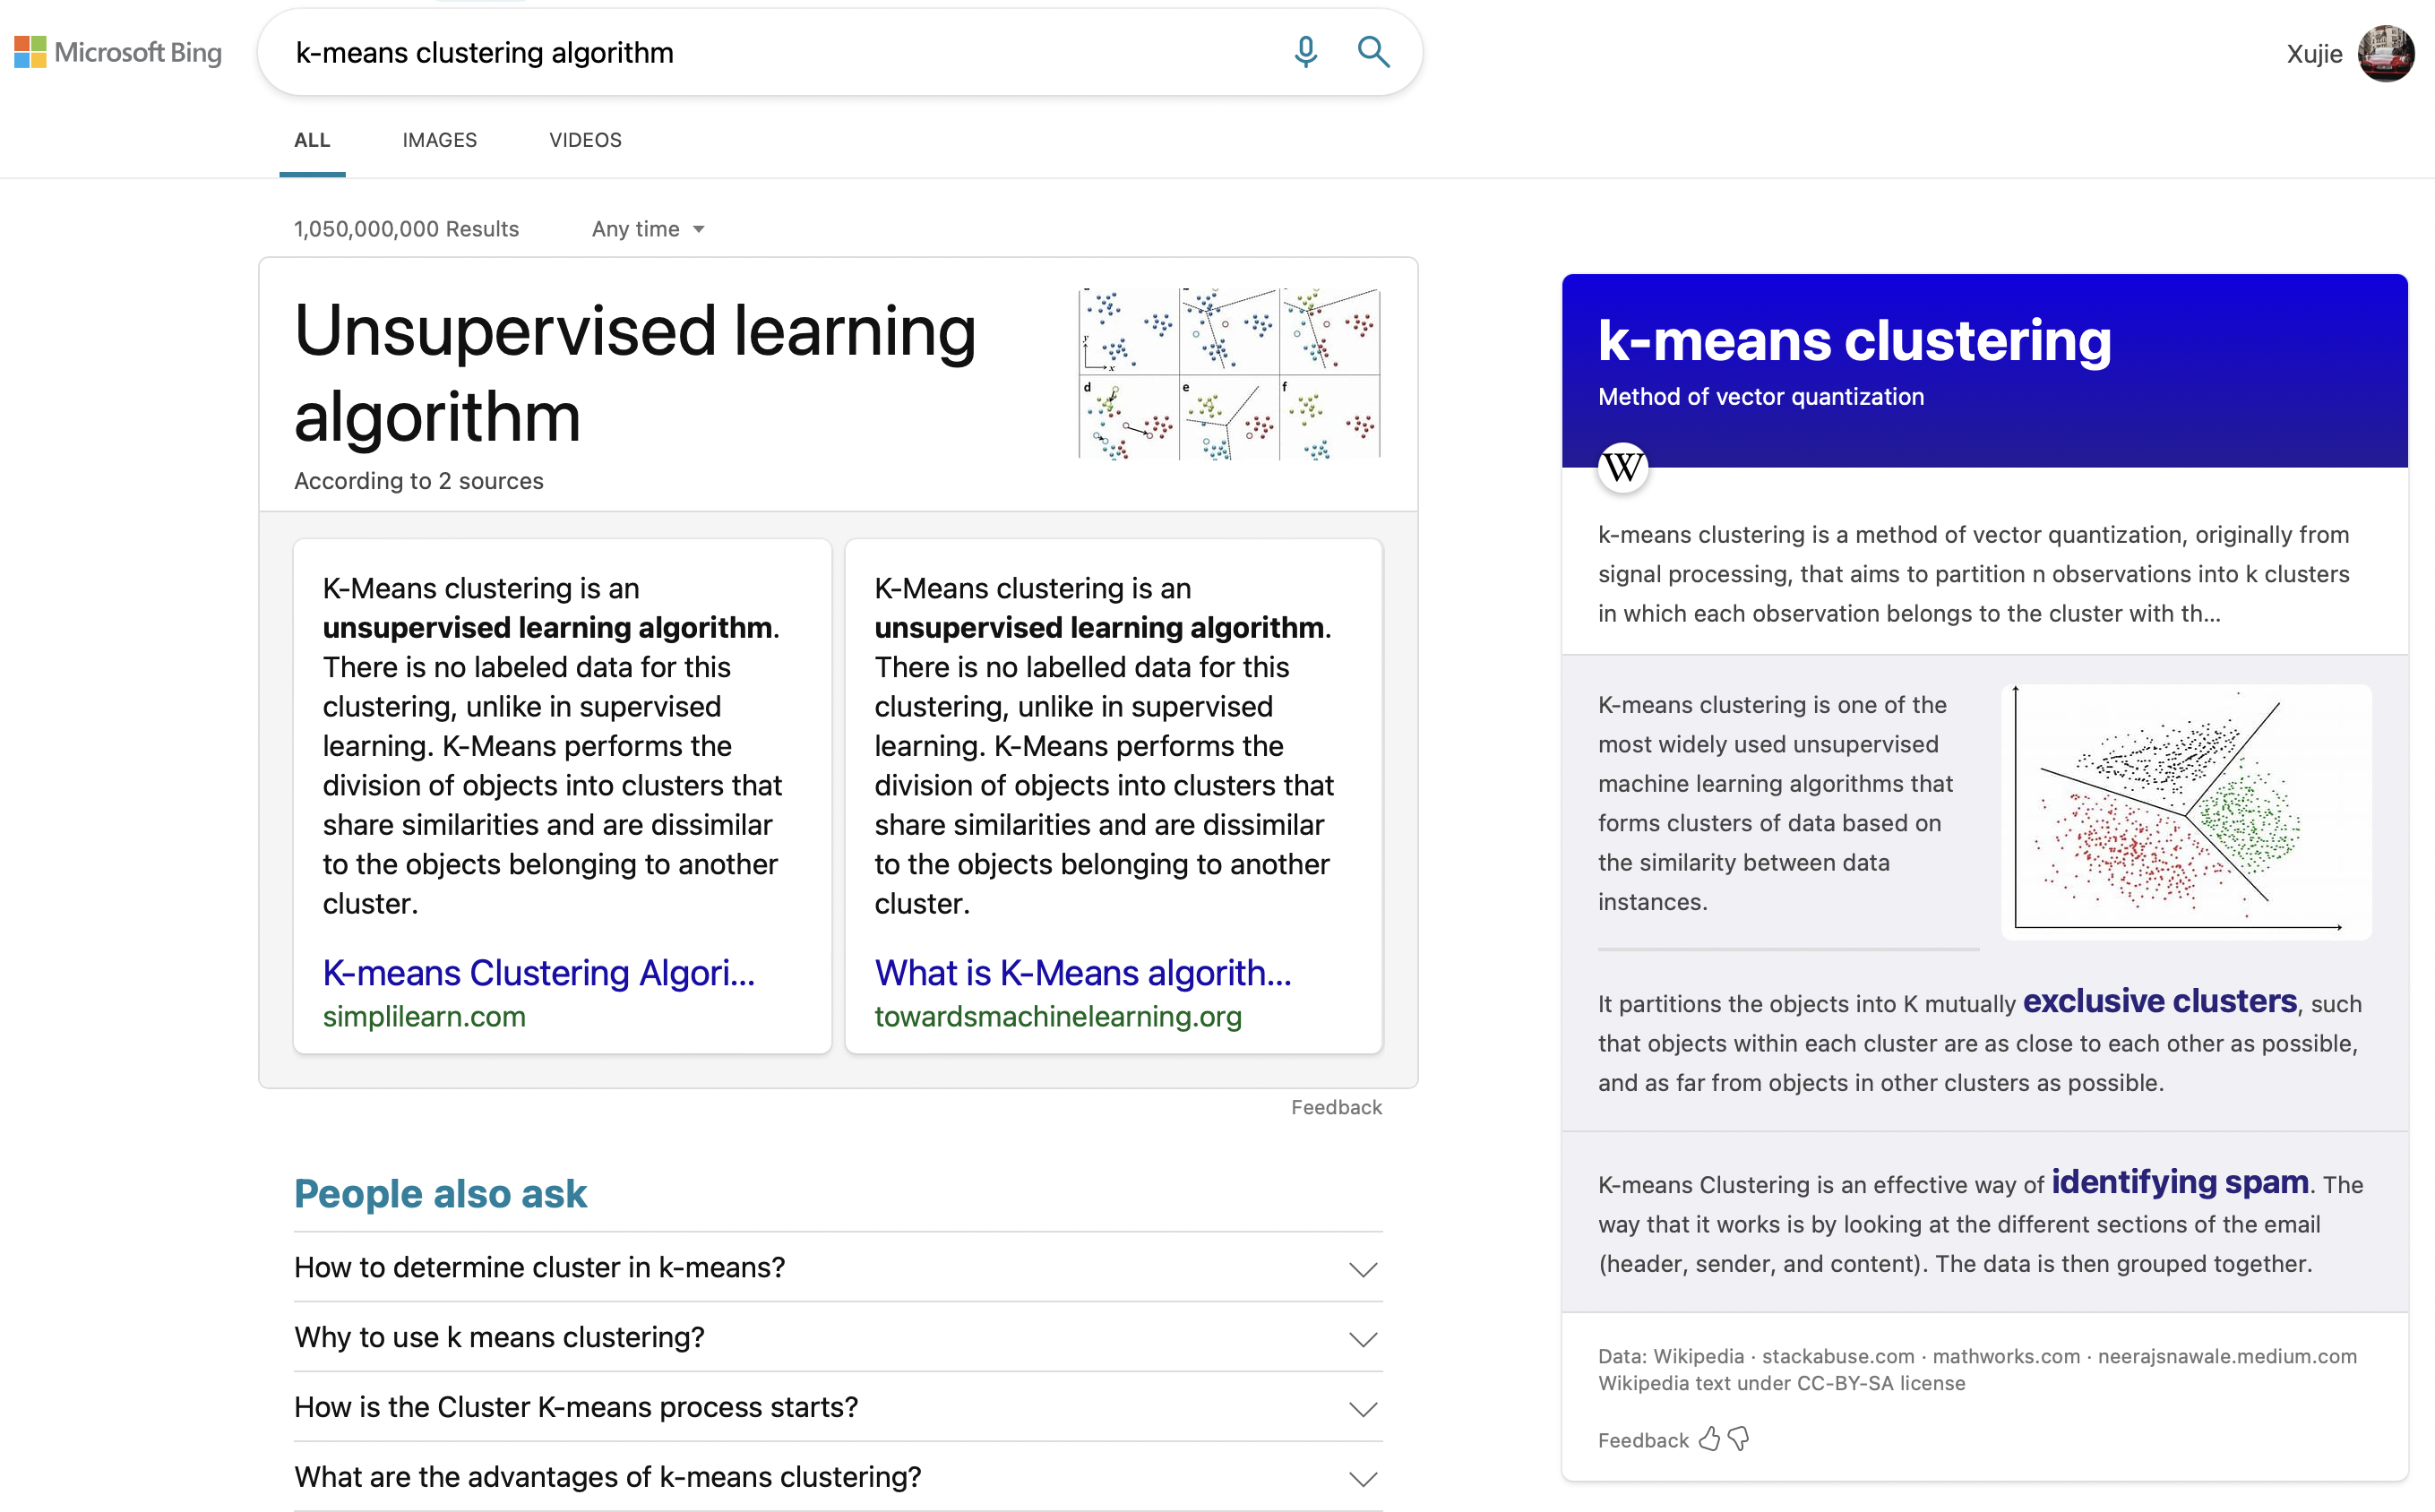
\includegraphics[width=0.8\textwidth]{Bing_home.png}
        \caption{Bing search results}
    \end{figure}
    As shown in Figure 4, Bing's search results are largely the same as Google's, except that there are no recommended academic articles at the top. However, as shown in Figure 5, the search results for related video content are displayed visually, and other keywords related to K-means clustering are also shown in the 'Explore more' section on the right.
    \begin{figure}[ht]
        \centering
        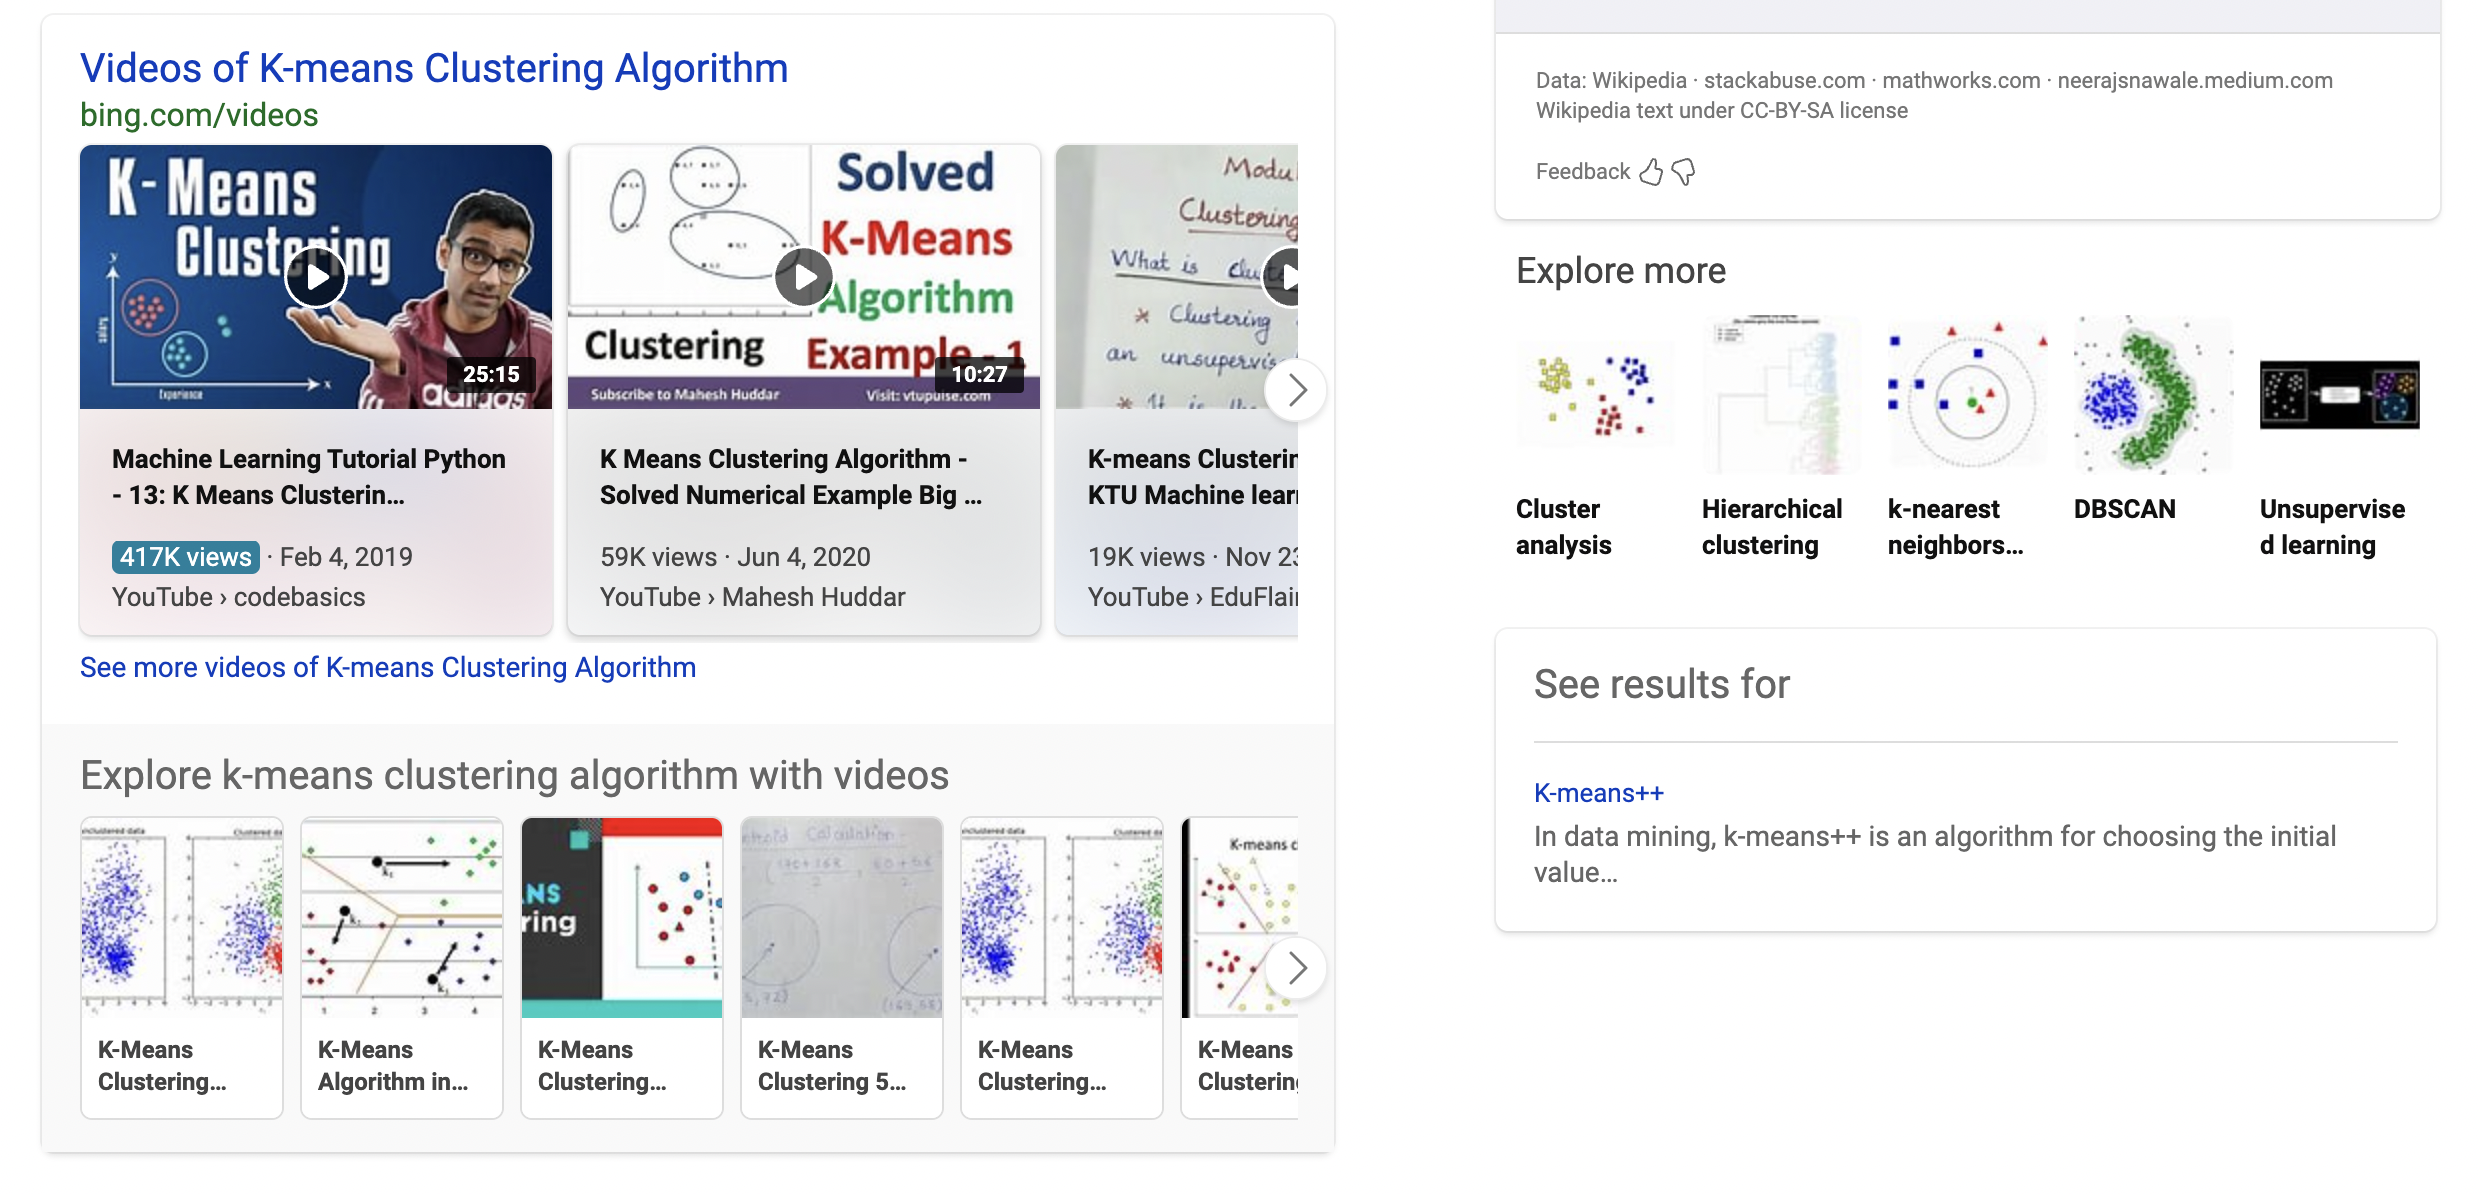
\includegraphics[width=0.8\textwidth]{Bing1.png}
        \caption{Bing related results}
    \end{figure}

    \section{Baidu search results}
    \begin{figure}[ht]
        \centering
        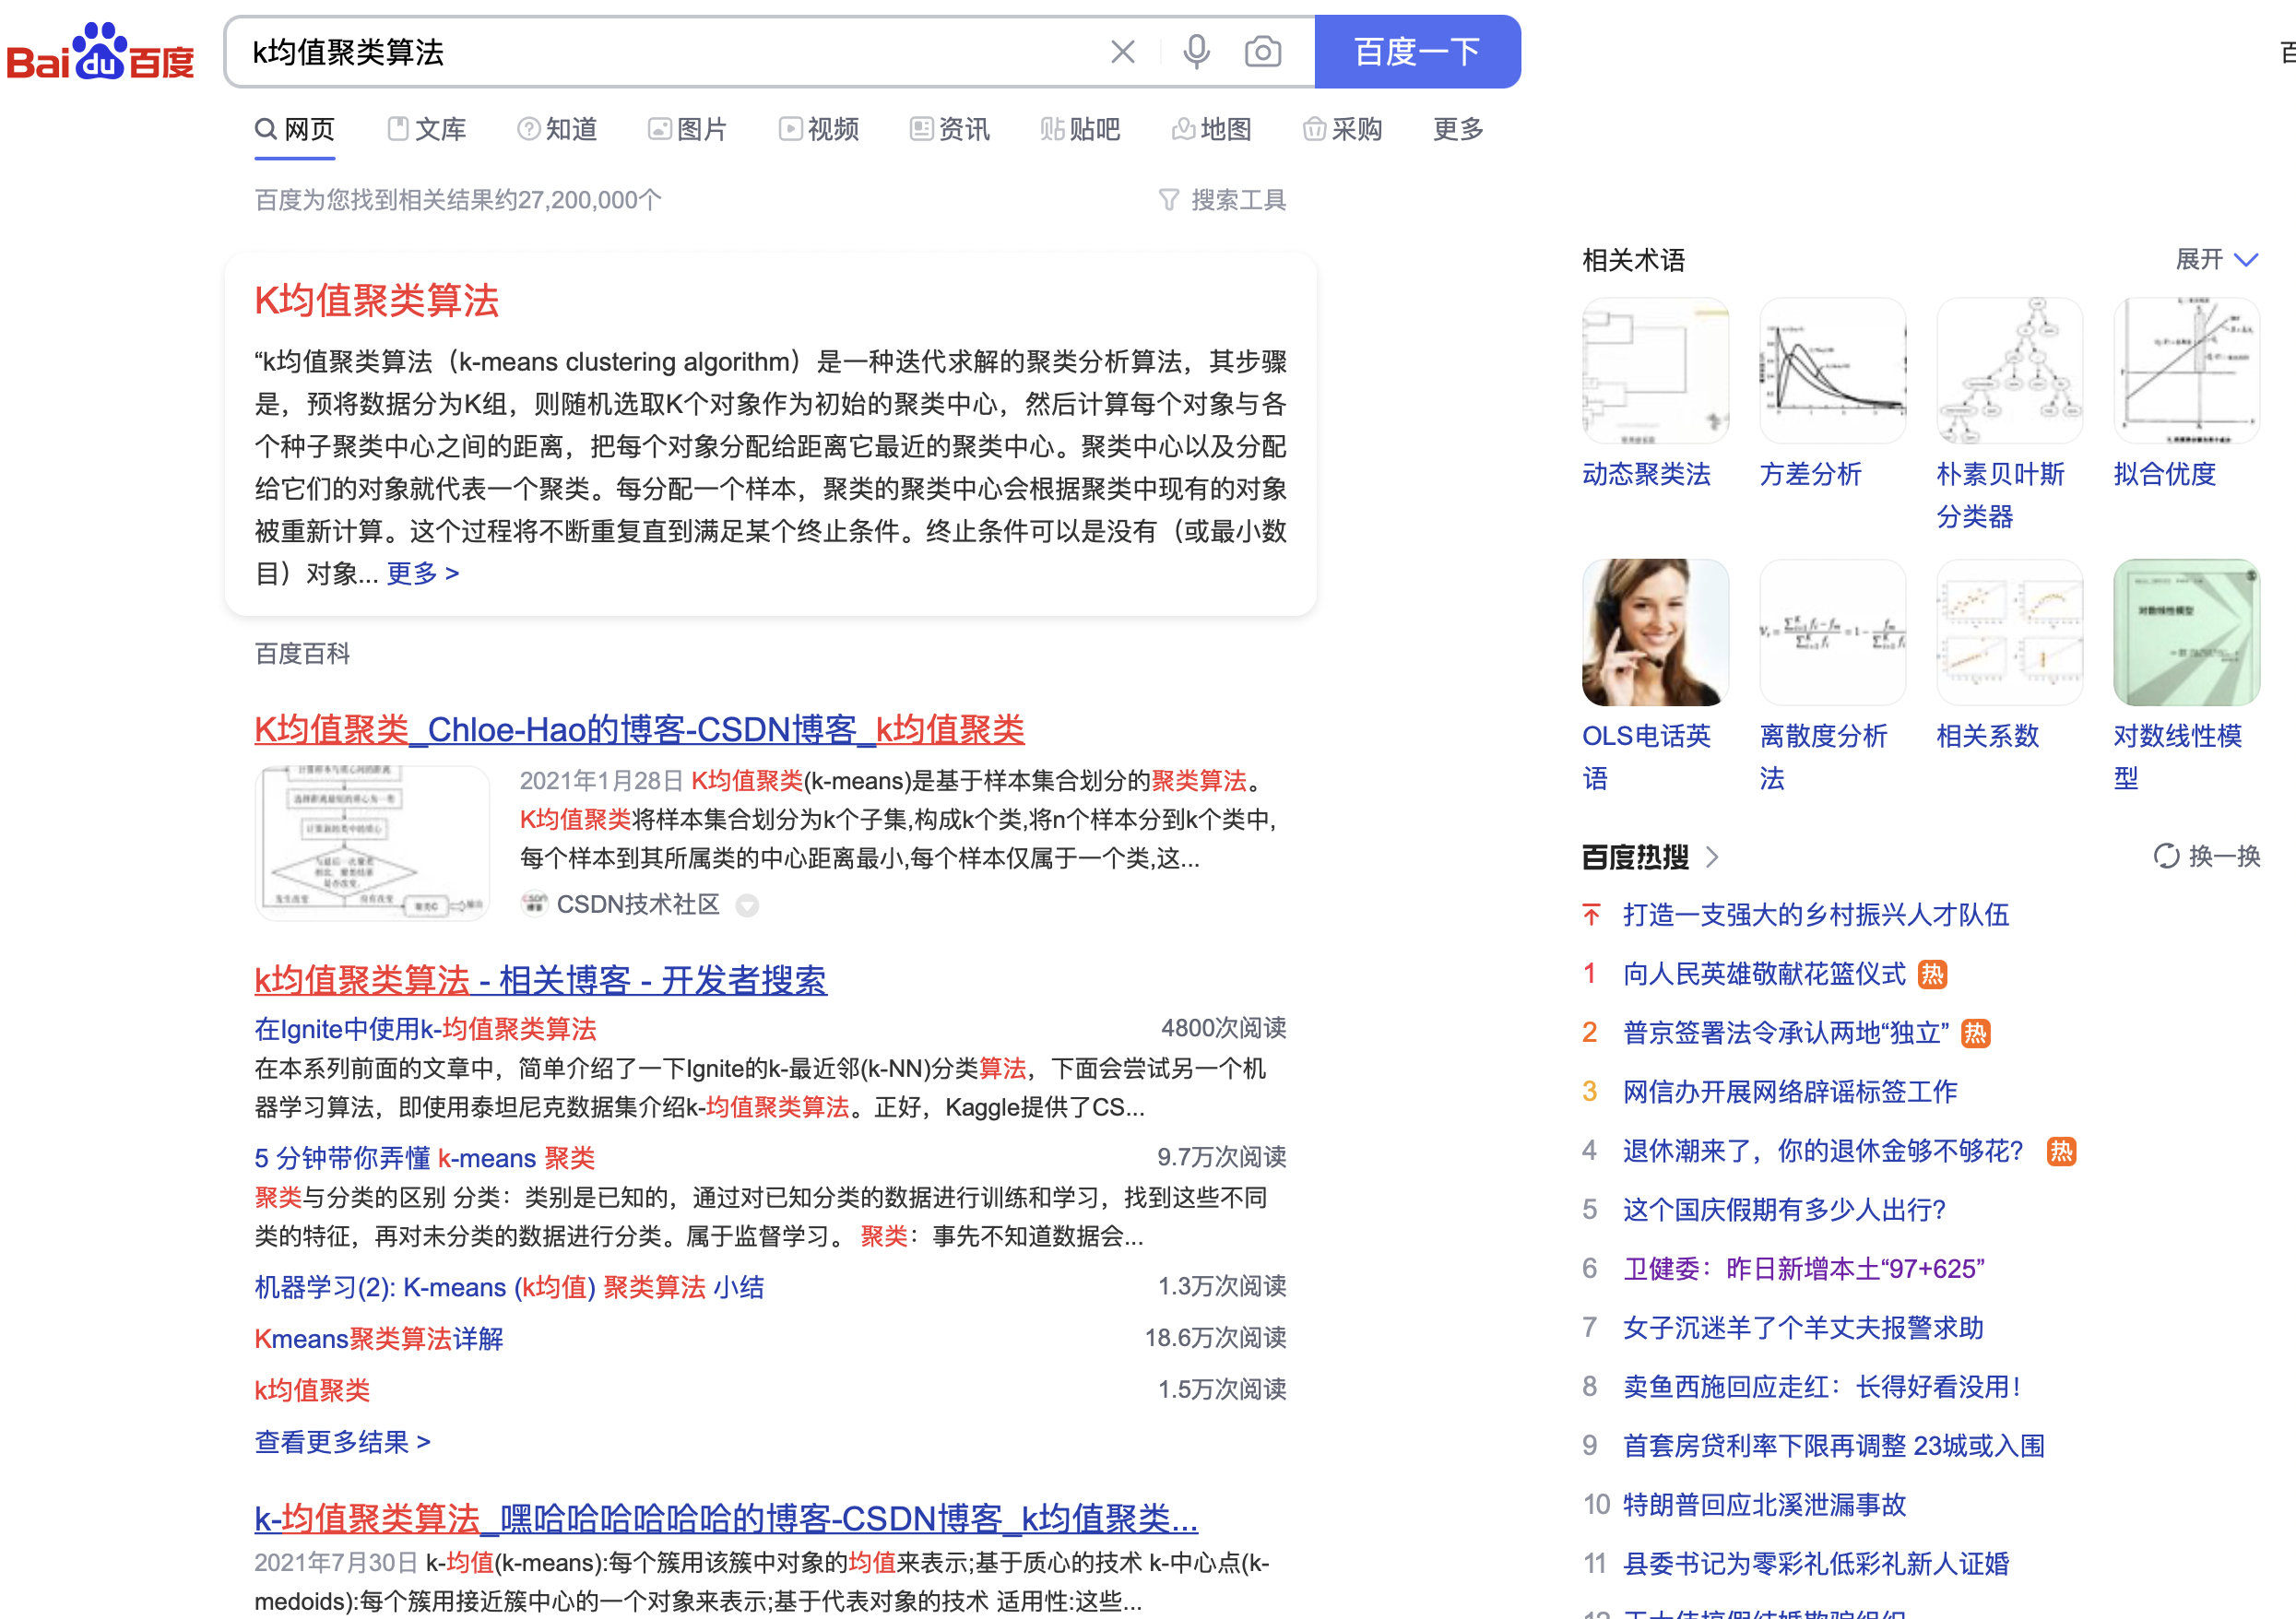
\includegraphics[width=0.8\textwidth]{Baidu_home.png}
        \caption{Baidu search results}
    \end{figure}
    As shown in Figure 6, Baidu's search results also have links to related profiles and associated terms. However, the specific search results are highly repetitive and of low quality, mostly from CSDN, as shown in Figure 7, I found that two results use the exact same image, but do not indicate the source, which is a very unprofessional behavior. And the right side of Baidu search will also appear "Baidu Hot Search" which is not related to K-means clustering.
    \begin{figure}[ht]
        \centering
        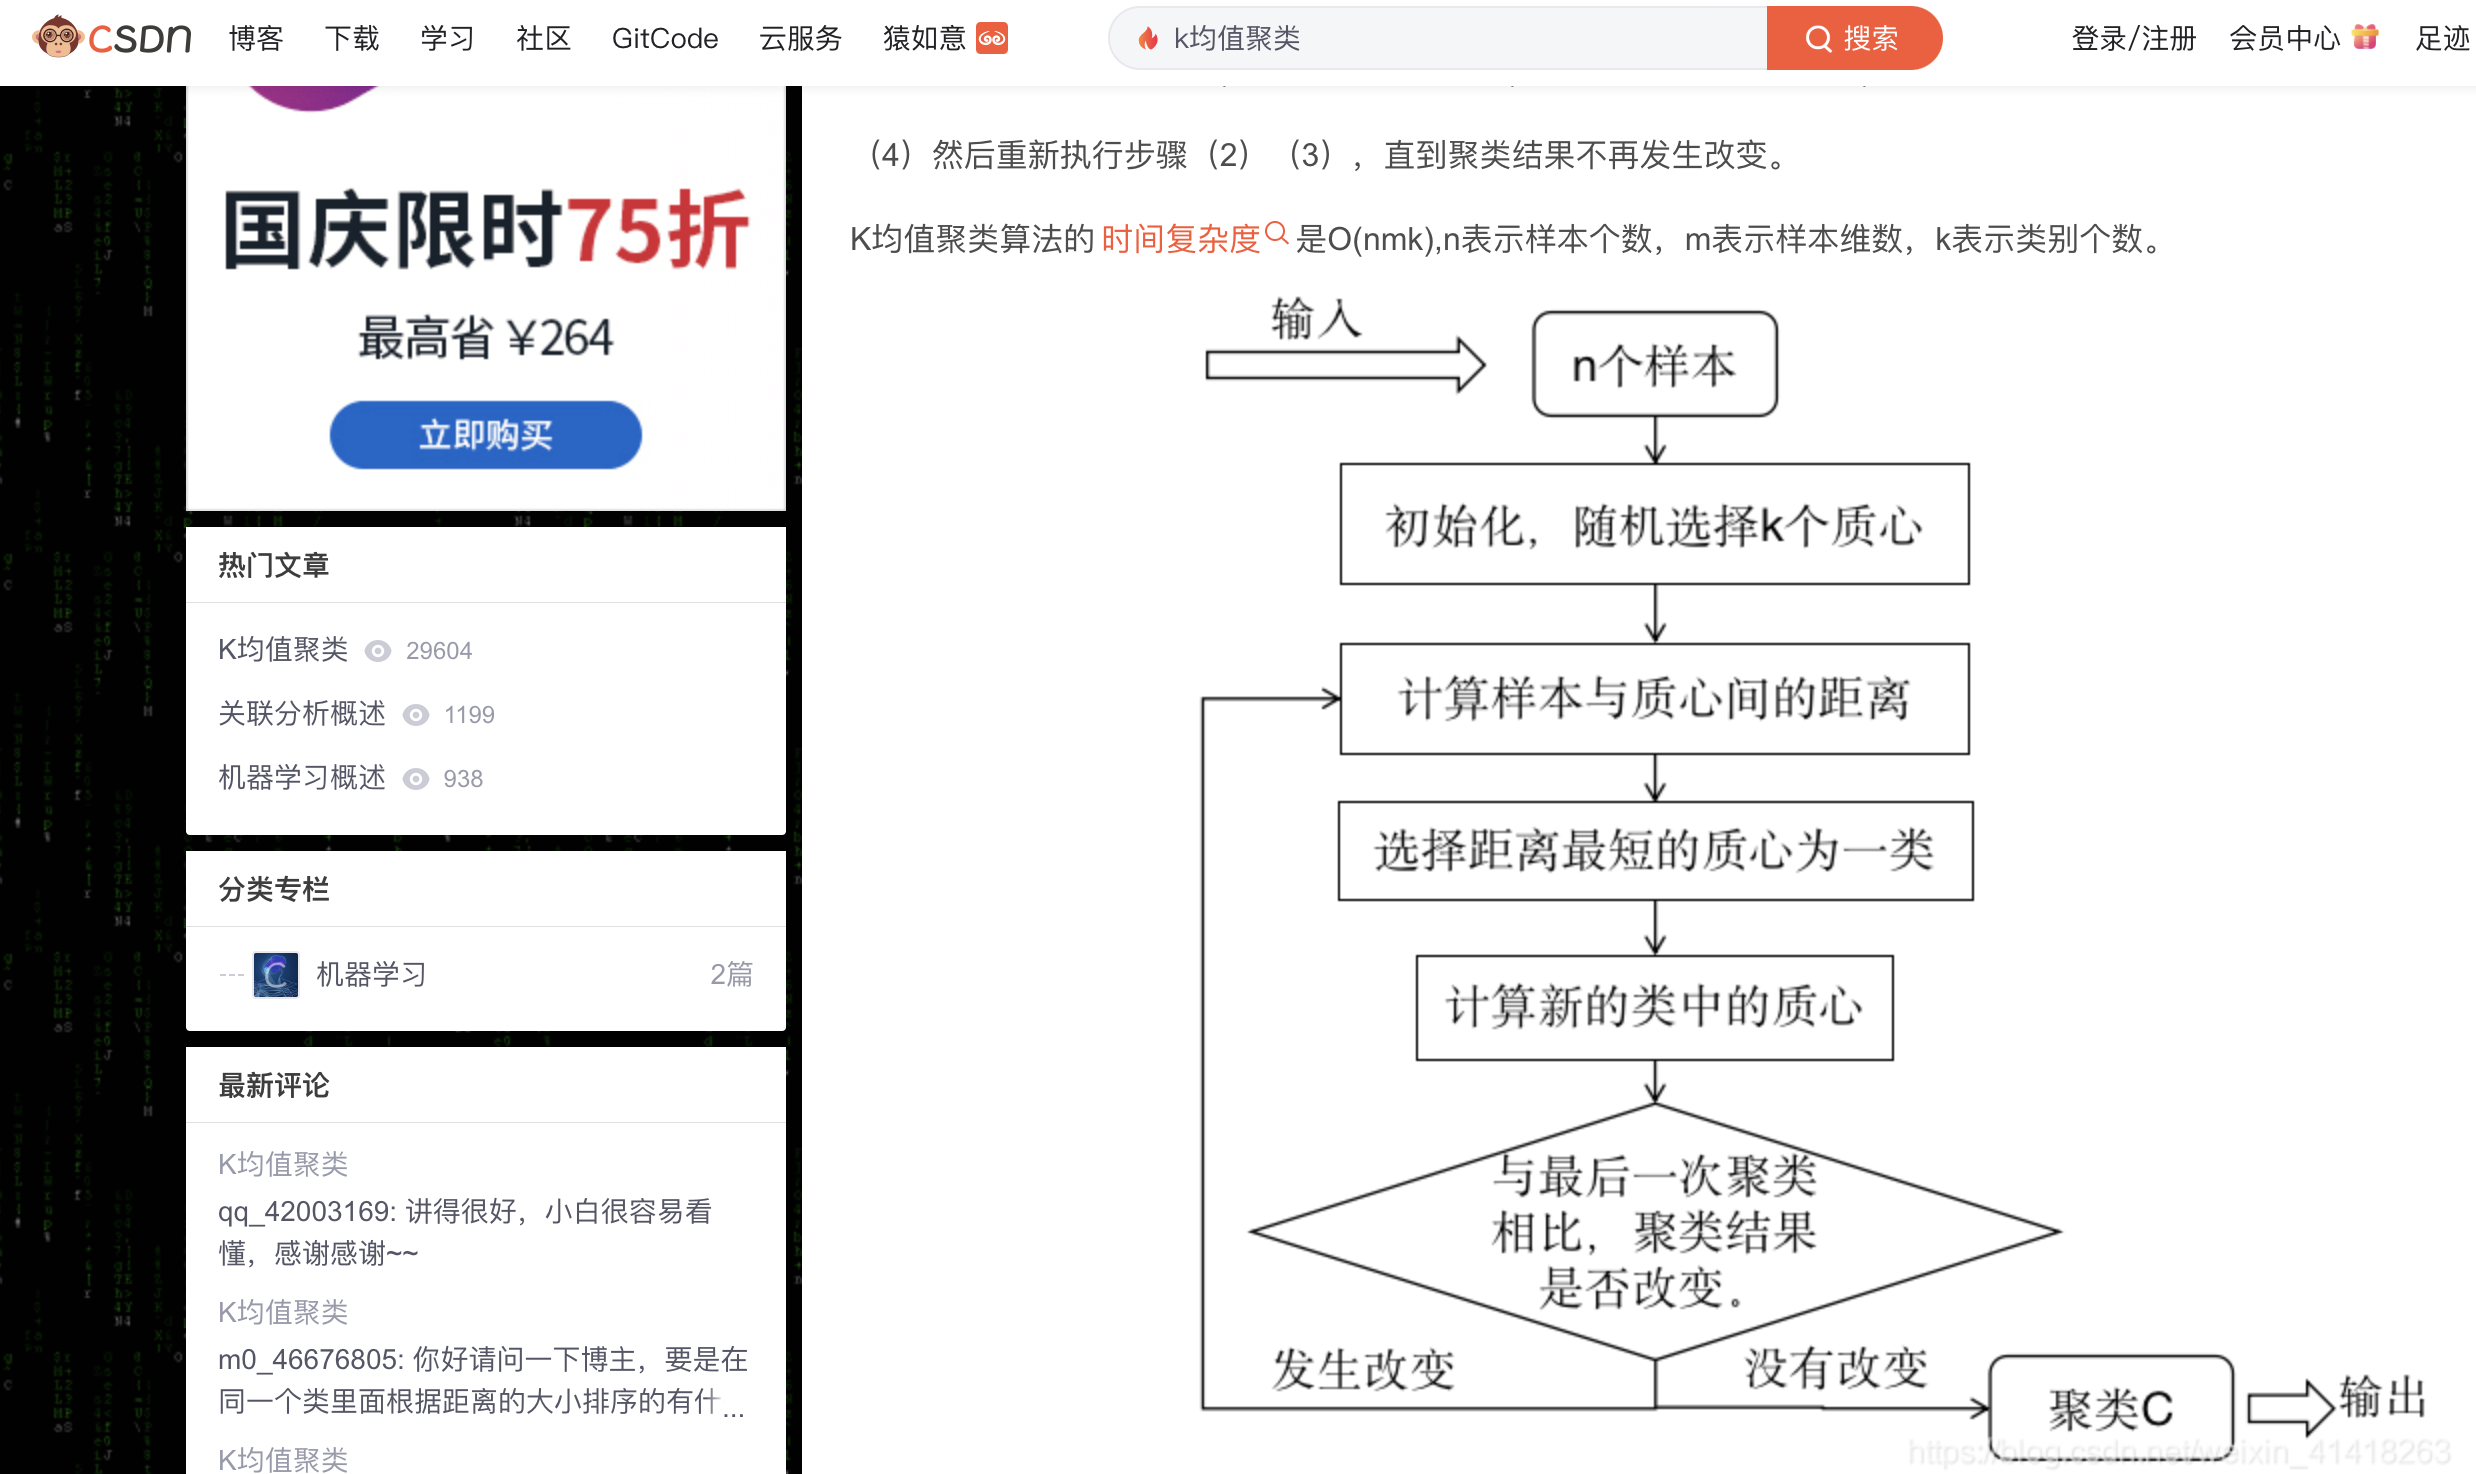
\includegraphics[width=0.8\textwidth]{Baidu1.png}
        \caption{CSDN result}
    \end{figure}

    \section{Conclusion}
    To sum up, Google and Bing's search results are concise, professional and rich in related information. Baidu's search results are of lower quality and have more interfering information. For professional knowledge-related search content, Google is still more recommended.

    \section{References}
\end{document}